%%%%%%%%%%%%%%%%%%%%%%% file template.tex %%%%%%%%%%%%%%%%%%%%%%%%%
%
% This is a template file for Web of Conferences Journal
%
% Copy it to a new file with a new name and use it as the basis
% for your article
%
%%%%%%%%%%%%%%%%%%%%%%%%%% EDP Science %%%%%%%%%%%%%%%%%%%%%%%%%%%%
%
%%%\documentclass[option]{webofc}
%%% "twocolumn" for typesetting an article in two columns format (default one column)
%
\documentclass{webofc}
\usepackage[varg]{txfonts}   % Web of Conferences font
\usepackage{listings}
\usepackage{xcolor}

\colorlet{punct}{red!60!black}
\definecolor{background}{HTML}{EEEEEE}
\definecolor{delim}{RGB}{20,105,176}
\colorlet{numb}{magenta!60!black}

\lstdefinelanguage{json}{
    basicstyle=\normalfont\ttfamily,
    numbers=left,
    numberstyle=\scriptsize,
    stepnumber=1,
    numbersep=8pt,
    showstringspaces=false,
    breaklines=true,
    frame=lines,
    backgroundcolor=\color{background},
    literate=
     *{0}{{{\color{numb}0}}}{1}
      {1}{{{\color{numb}1}}}{1}
      {2}{{{\color{numb}2}}}{1}
      {3}{{{\color{numb}3}}}{1}
      {4}{{{\color{numb}4}}}{1}
      {5}{{{\color{numb}5}}}{1}
      {6}{{{\color{numb}6}}}{1}
      {7}{{{\color{numb}7}}}{1}
      {8}{{{\color{numb}8}}}{1}
      {9}{{{\color{numb}9}}}{1}
      {:}{{{\color{punct}{:}}}}{1}
      {,}{{{\color{punct}{,}}}}{1}
      {\{}{{{\color{delim}{\{}}}}{1}
      {\}}{{{\color{delim}{\}}}}}{1}
      {[}{{{\color{delim}{[}}}}{1}
      {]}{{{\color{delim}{]}}}}{1},
}

\lstdefinelanguage{httprequest}{
    basicstyle=\normalfont\ttfamily,
    numbers=left,
    numberstyle=\scriptsize,
    stepnumber=1,
    numbersep=8pt,
    showstringspaces=false,
    breaklines=true,
    frame=lines,
    backgroundcolor=\color{background}
}

%
% Put here some packages required or/and some personnal commands
%
%
\begin{document}
%
\title{Capability-Based Authorization for HEP}
%
% subtitle is optionnal
%
%%%\subtitle{Do you have a subtitle?\\ If so, write it here}

\author{\firstname{Derek} \lastname{Weitzel}\inst{1}\fnsep\thanks{\email{dweitzel@cse.unl.edu}} \and
        \firstname{Brian} \lastname{Bockelman}\inst{1}\fnsep\thanks{\email{bbockelm@cse.unl.edu}} \and
        \firstname{Jim} \lastname{Basney}\inst{2} \and 
        \firstname{Todd} \lastname{Tannenbaum}\inst{3} \and 
        \firstname{Zach} \lastname{Miller}\inst{3}
        % etc.
}

\institute{University of Nebraska - Lincoln 
\and
           NCSA
\and
           University of Wisconsin-Madison
          }

\abstract{%
Outside the HEP computing ecosystem, it is vanishingly rare to encounter user X509 certificate authentication (and proxy certificates are even more rare). The web never widely adopted the user certificate model, but increasingly sees the need for federated identity services and distributed authorization. For example, Dropbox, Google and Box instead use bearer tokens issued via the OAuth2 protocol to authorize actions on their services. Thus, the HEP ecosystem has the opportunity to reuse recent work in industry that now covers our needs. We present a token-based ecosystem for authorization tailored for use by CMS.

We base the tokens on the SciTokens profile for the standardized JSON Web Token (JWT) format. The token embeds a signed description of what capabilities the VO grants the bearer; the site-level service can verify the VO’s signature without contacting a central service.

In this paper, we describe the modifications done to enable token-based authorization in various software packages used by CMS, including XRootD, CVMFS, and HTCondor. We describe the token-issuing workflows that would be used to get tokens to running jobs in order to authorize data access and file stageout, and explain the advantages for hosted web services. Finally, we outline what the transition would look like for an experiment like CMS.

}
%
\maketitle
%
\section{Introduction}
\label{intro}

Capability-based authorization provides an opportunity to reuse technology industry standards and software for High Energy Physics.  They provide stuff

At the core of today's grid security infrastructure is the concept of \textit{identity} and \textit{impersonation}.

\begin{itemize}
    \item A grid certificate provides you with a globally recognized identification
    \item The grid proxy allows a third party to impersonate you on your behalf.
    \item The remote service maps your identity to a set of locally defined authorizations
\end{itemize}

A grid certificate is a X509 \cite{housley1998internet} 

% Talk about advantages of capability based



% Identity vs. capability
The High Energy Physics community, as well as the research infrastructures it relies on, use the X509 certificate for authentication.  The X509


\subsection{Public Key}





% Should we even have a background section?
\section{Background}
\label{background}

\subsection{OAuth}
\label{sec:oauth}

OAuth is a workflow that allows for user to authorize a third party to perform actions on it's behalf.  It is widely used in 


\subsection{X509}
\label{sec:x509}

\section{Implementation}
\label{sec:implementation}

% We had to modify several pieces of software.  Including:
% XRootD For file transfer services
% CVMFS for ease of use for reading
% HTCondor to create and maintain tokens
Various technologies had to be modified to utilize capability tokens.  Within a workflow, capability tokens need to flow from the user to the the job.  

\begin{figure}[ht]
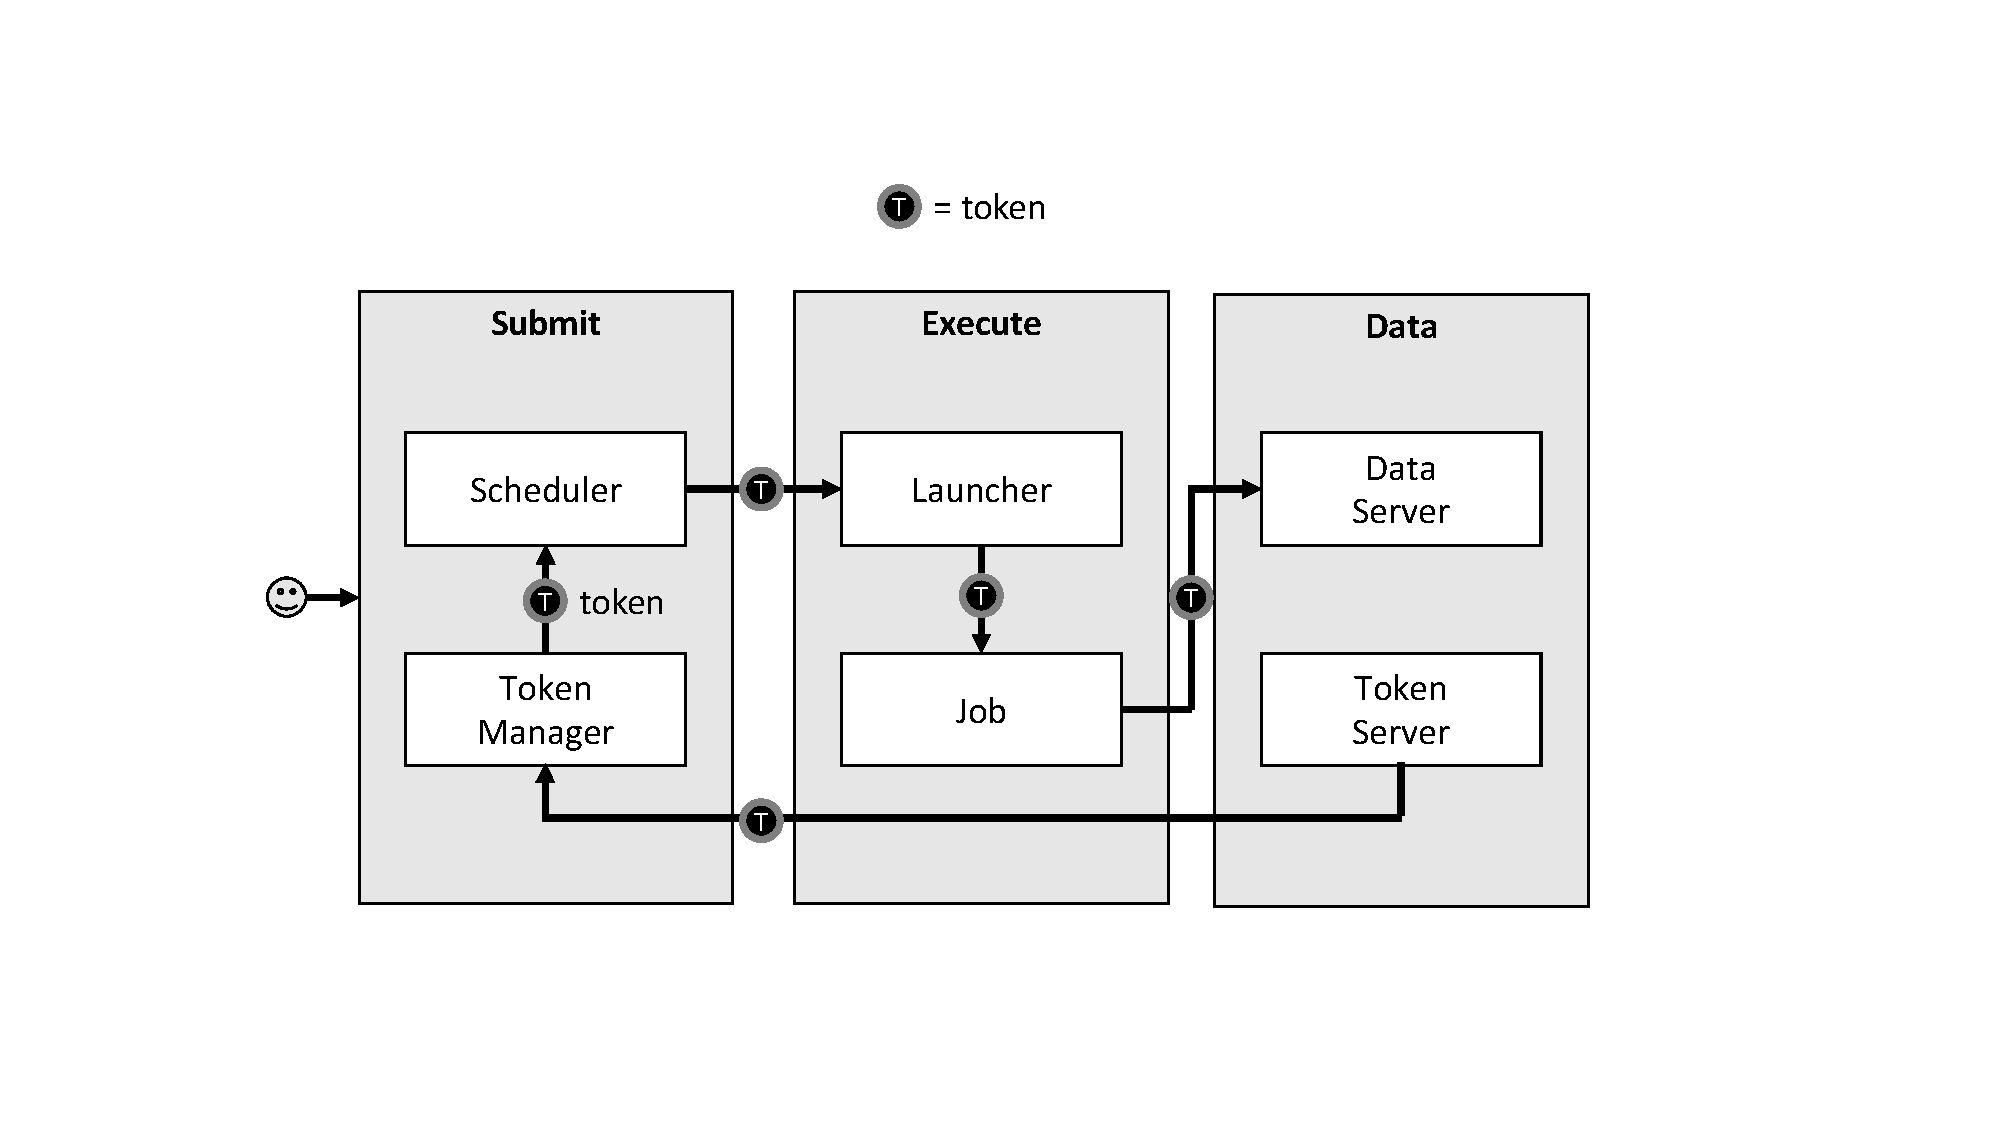
\includegraphics[width=\textwidth]{images/SciTokensFlow.pdf}
\caption{Token flow in a workflow}
\label{fig:tokenflow}
\end{figure}

Figure \ref{fig:tokenflow} shows the flow of a token through a workflow.  The token is first retrieved from a token server.  The token manager will manage the token on behalf of the user, retrieving refreshed tokens when the current token expires.  The scheduler will send the token to the execute host.  The execute host will make the token available to the job, which will use it to access resources such as data.

Each step of this workflow required modifications software that is used on the Grid.  HTCondor \cite{condor-practice} was enhanced in order to retrieve and refresh tokens on behalf of the user.  XRootD \cite{dorigo2005xrootd} and CVMFS \cite{buncic2010cernvm} where modified to accept and validate tokens to access data.

XRootD and CVMFS both use the SciTokens library \cite{scitokens-lib}, described in \ref{sec:scitokenslib} to validate and authorized tokens.


\subsection{SciTokens Library}
\label{sec:scitokenslib}
SciTokens \cite{withers2018scitokens} provides a library that is used to create and validate scitokens.  A SciToken is a JSON Web Token \cite{jones2015json} with attributes that describe how a token can be used.

% JWT overview

\begin{figure}[ht]
\begin{lstlisting}[language=json,firstnumber=1]
{
  "typ": "JWT",
  "alg": "RS256",
  "kid": "key-rs256"
}
{
  "scope": "read:/protected",
  "aud": "example.com",
  "iss": "https://demo.scitokens.org",
  "exp": 1539652082,
  "iat": 1539651482,
  "nbf": 1539651482,
  "jti": "76a3c07f-1e9d-4441-a3e2-6f37dbe26327"
}
\end{lstlisting}
\caption{Example SciToken}
\label{fig:scitoken}
\end{figure}

Figure \ref{fig:scitoken} shows an example SciToken.  The special attribute \texttt{scope} is used to describe how the token can be used.  In this example, the token can be used to read from the resource at \texttt{/protected}.

The library can be used to validate the signature of the token.  It can also be used to query the token for authorizations.

% Include workflow graphic, if not already in intro

\subsection{XRootD}
\label{sec:xrootd}

XRootD is a high performance data server.  We modified XRootD to pass an authorization header to a plugin.  We wrote a plugin \cite{xrootd-scitokens} that would use the SciTokens library to validate the incoming token.

The plugin uses Boost \cite{dawes2009boost} to connect the C++ API of XRootD to the Python API of the SciTokens library.  XRootD passes the token to the plugin which creates an Access Control List of directories this token is allowed to access.  XRootD will cache the ACL until the token expires.

\begin{figure}[ht]
\begin{lstlisting}[language=httprequest,firstnumber=1]
GET /store/path HTTP/1.1
Host: storage.site1.com
Authorization: Bearer eyJ0eXAiOiJKV1...
\end{lstlisting}
    \caption{Example HTTP Request with Token}
    \label{fig:examplerequest}
\end{figure}

Figure \ref{fig:examplerequest} shows an example HTTP request including the token.  The token is used in the \texttt{Authorization} line, and it is treated as a bearer token \cite{jones2012oauth}.  The bearer token is encoded in base64 encoding \cite{josefsson2006base16}.  XRootD will pass the \texttt{Authorization} header to the token plugin for validation and to create the ACLs.

\subsection{CVMFS}
\label{sec:cvmfs}

Cern-VM FileSystem (CVMFS) is a read-only global data source.  It is mounted on execute hosts as a traditional filesystem, making it easier to use than a remote storage system.

% External repos
CVMFS has the capability to use external sources as the data repository.  The metadata for files such as size, name, and checksums are stored within the CVMFS namespace.  The contents of the files are stored on external servers reachable from CVMFS through an HTTP interface.  When a user requests the contents of a file, CVMFS will request the data from a list of potential external servers.

% Forwarding the tokens
In order to authenticate with the external servers, a token must be passed from the user to the data server.  A token is stored within the user's environment and pointed to by an environment variable.  When a request for data that is protected by tokens is requested by CVMFS, it will start a separate process that will retrieve the token from the user's environment and validate it.  Once CVMFS has the token, it will use it to authenticate with the remote server and request the data. 

\subsection{HTCondor}
\label{sec:htcondor}

HTCondor is a job and workflow management system.  Support for Tokens, specifically OAuth 2.0 \cite{hardt2012oauth} tokens, where added to different components in the system, as seen in Figure \ref{fig:htcondorflow}.

\begin{figure}[ht]
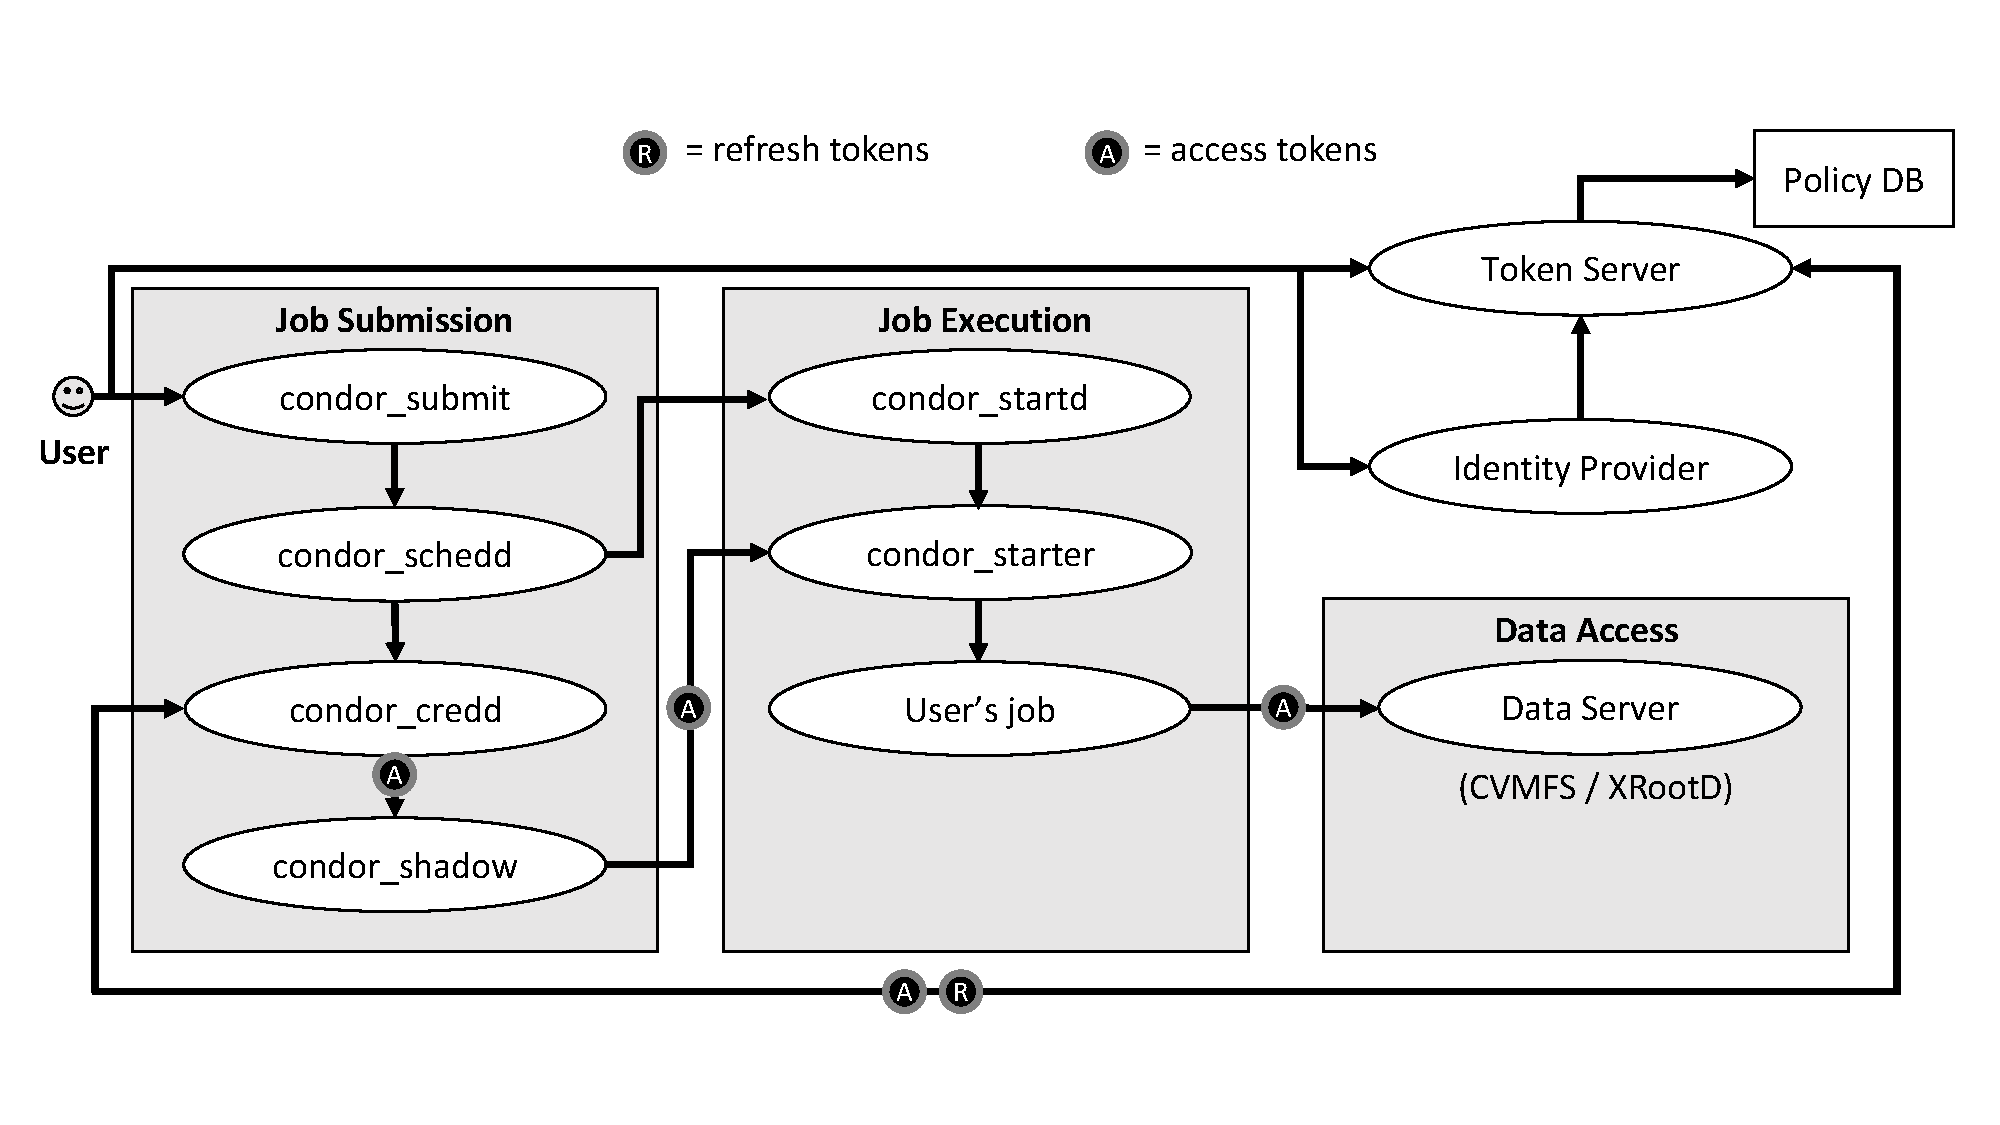
\includegraphics[width=\textwidth]{images/HTCondorTokenFlow.pdf}
\caption{Token flow through HTCondor system}
\label{fig:htcondorflow}
\end{figure}

\noindent
Figure \ref{fig:htcondorflow} shows the token flow within the HTCondor system.

\begin{enumerate}
    \item The user first submits the job using the tool \texttt{condor\_submit}.
    \item The user is redirected to the token server and identity provider, which authorizes the users and creates a token for with the authorization requested.
    \item The token and the refresh token is stored by the \texttt{condor\_credd}.  
    \item The token is sent to the job through the \texttt{condor\_shadow} and the \texttt{condor\_shadow}.
    \item The user's job can use the token to access data on the data server.
\end{enumerate}

The \texttt{condor\_credd} manages the token credential throughout the lifetime of the workflow.  Periodically, it will use the refresh token to retrieve a new token from the token server.  The token is only valid for a short time, while the refresh token could be valid for months.  The \texttt{condor\_credd} will refresh the token before the expiration and send the updated token to the jobs.



\section{Evaluation}
\label{sec:eval}

\section{Conclusion}
\label{sec:conclusion}



%
% BibTeX or Biber users please use (the style is already called in the class, ensure that the "woc.bst" style is in your local directory)
\bibliography{main}

\end{document}

% end of file template.tex
